% Created 2019-12-07 lø 18:59
% Intended LaTeX compiler: pdflatex
\documentclass[12pt]{article}

%%%% settings when exporting code %%%% 

\usepackage{listings}
\lstset{
backgroundcolor=\color{white},
basewidth={0.5em,0.4em},
basicstyle=\ttfamily\small,
breakatwhitespace=false,
breaklines=true,
columns=fullflexible,
commentstyle=\color[rgb]{0.5,0,0.5},
frame=single,
keepspaces=true,
keywordstyle=\color{black},
literate={~}{$\sim$}{1},
numbers=left,
numbersep=10pt,
numberstyle=\ttfamily\tiny\color{gray},
showspaces=false,
showstringspaces=false,
stepnumber=1,
stringstyle=\color[rgb]{0,.5,0},
tabsize=4,
xleftmargin=.23in,
emph={anova,apply,class,coef,colnames,colNames,colSums,dim,dcast,for,ggplot,head,if,ifelse,is.na,lapply,list.files,library,logLik,melt,plot,require,rowSums,sapply,setcolorder,setkey,str,summary,tapply},
emphstyle=\color{blue}
}

%%%% packages %%%%%

\usepackage[utf8]{inputenc}
\usepackage[T1]{fontenc}
\usepackage{lmodern}
\usepackage{textcomp}
\usepackage{color}
\usepackage{enumerate}
\usepackage{graphicx}
\usepackage{grffile}
\usepackage{wrapfig}
\usepackage{rotating}
\usepackage{longtable}
\usepackage{multirow}
\usepackage{multicol}
\usepackage{changes}
\usepackage{pdflscape}
\usepackage{geometry}
\usepackage[normalem]{ulem}
\usepackage{amssymb}
\usepackage{amsmath}
\usepackage{amsfonts}
\usepackage{dsfont}
\usepackage{array}
\usepackage{ifthen}
\usepackage{hyperref}
\usepackage{natbib}
\pagestyle{empty} % no page numbering
\usepackage[french, english]{babel}
\newcommand{\Rlogo}{\textbf{\textsf{R}}}
\newcommand{\Cpp}{C\nolinebreak\hspace{-.05em}\raisebox{.4ex}{\tiny\bf +}\nolinebreak\hspace{-.10em}\raisebox{.4ex}{\tiny\bf +}}
\usepackage{eurosym} % euro symbol
\usepackage{titlesec}
\titleformat{\section}{\large}{\thesection}{1em}{}
\titlespacing*{\section}{0pt}{0.25\baselineskip}{0.25\baselineskip}
\geometry{
left=20mm,
right=20mm,
top=20mm,
bottom=20mm
}
\RequirePackage{setspace} % to modify the space between lines - incompatible with footnote in beamer
\renewcommand{\baselinestretch}{1.1}
\usepackage{framed}
\usepackage{tocloft}
\newlength{\outerbordwidth}
\raggedbottom
\raggedright
\setlength{\outerbordwidth}{3pt}  % Width of border outside of title bars
\definecolor{shadecolor}{gray}{0.75}  % Outer background color of title bars (0 = black, 1 = white)
\definecolor{shadecolorB}{gray}{0.93}  % Inner background color of title bars
\usepackage{mdframed}
\newcommand{\resitem}[1]{\item #1 \vspace{-2pt}}
\newcommand{\resheading}[1]{
\vspace{8pt}
\parbox{\textwidth}{\setlength{\FrameSep}{\outerbordwidth}
\begin{shaded}
\setlength{\fboxsep}{0pt}\framebox[\textwidth][l]{\setlength{\fboxsep}{4pt}\fcolorbox{shadecolorB}{shadecolorB}{\textbf{\sffamily{\mbox{~}\makebox[6.762in][l]{\large #1} \vphantom{p\^{E}}}}}}
\end{shaded}
}\vspace{-5pt}
}
\newcommand{\ressubheading}[4]{
\begin{tabular*}{6.5in}{l@{\cftdotfill{\cftsecdotsep}\extracolsep{\fill}}r}
\textbf{#1} & #2 \\
\textit{#3} & \textit{#4} \\
\end{tabular*}\vspace{-6pt}}
\usepackage{bibentry}
\nobibliography*
\newcommand{\myname}[1]{\textbf{#1}}
\usepackage{url}
\date{\today}
\title{}
\hypersetup{
 colorlinks=true,
 citecolor=[rgb]{0,0.5,0},
 urlcolor=[rgb]{0,0,0.5},
 linkcolor=[rgb]{0,0,0.5},
 pdfauthor={Brice Ozenne},
 pdftitle={},
 pdfkeywords={},
 pdfsubject={},
 pdfcreator={Emacs 25.2.1 (Org mode 9.0.4)},
 pdflang={English}
 }
\begin{document}

\begin{tabular*}{7in}{l@{\extracolsep{\fill}}r}
	\textbf{\Large Brice Ozenne} & \textbf{\today} \\
\end{tabular*}

\bigskip

\begin{minipage}{0.2\linewidth}
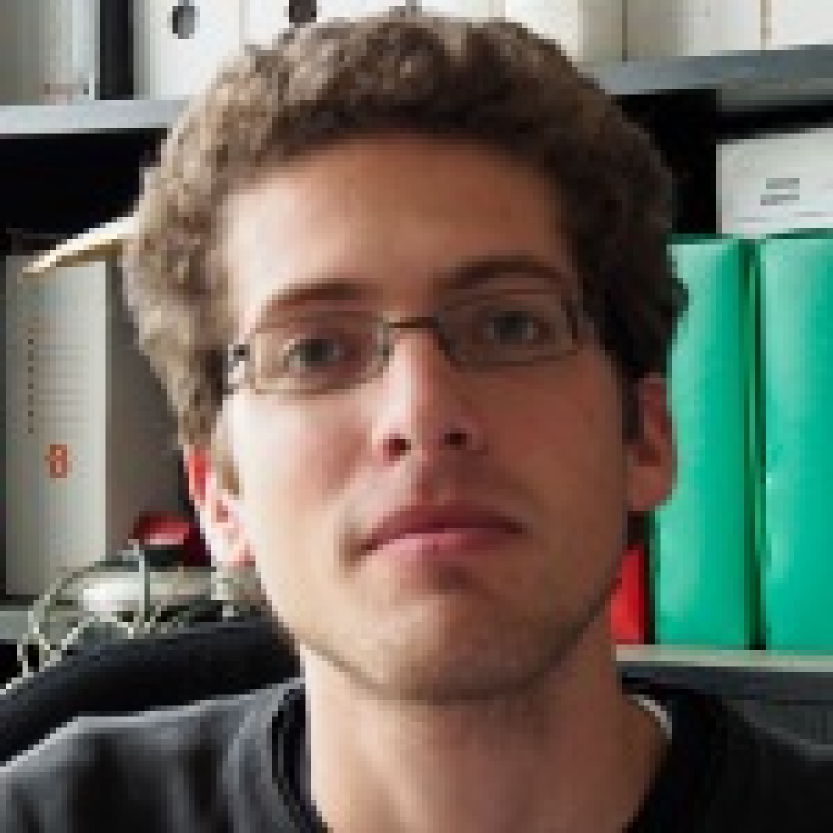
\includegraphics[width=\linewidth]{photoId.png}
\end{minipage}
\begin{minipage}{0.75\linewidth}
\begin{tabular*}{7in}{ll@{ }l}
	Nationality&:& french  \\
	Date of birth&:& February 8, 1990  \\
	Personal email&:& \url{brice.mh.ozenne@gmail.com} \\ 
	Personal phone number&:& (+45) 52 328 128 \\ 
        Personal address&:& Nordre Teglkaj 18, 5 t.h., 2450 Copenhagen SV, Denmark \\
\end{tabular*}
\end{minipage}

\bigskip

\resheading{CURRENT POSITION}
\begin{tabular}{l@{ }l}
	November 2015- Now:& \textbf{Postdoctoral researcher} (\href{http://publichealth.ku.dk/staff/?pure=en/persons/540231}{website})\\
	& Section of Biostatistics, University of Copenhagen \\
	& \O{}ster Farimagsgade 5, 1014 Copenhague, Danemark \\ [2mm]
	& Neurobiology Research Unit \\
	& Copenhagen University Hospital, Rigshospitalet \\
	& Building 6931, Blegdamsvej 9, DK-2100 Copenhagen, Denmark
\end{tabular}

\bigskip
My research work is organized around three topics:
\begin{itemize}
\item the development of \textbf{latent variable models} for the analysis of
complex data (software \texttt{lavaSearch2}). I apply these developments on
neuroimaging data and data from psychological tests to investigate
the relationship between the brain response and depression.
\end{itemize}

\smallskip

\begin{itemize}
\item the analysis of registry data with \textbf{time to events outcomes} and
\textbf{competing risks} (software \texttt{riskRegression}). My developments have,
for instance, been applied to compare preventive stroke treatments
using the danish registry data.
\end{itemize}

\smallskip

\begin{itemize}
\item the development of \textbf{generalized pairwise comparisons} to handle
multiple and heterogenous outcomes (software \texttt{BuyseTest}). A typical
application is the assessment of new chemotherapy where being able
to balance the benefit (longer in survival time) and the risk
(treatment side effects) in an interpretable way is important.
\end{itemize}

\resheading{SKILLS}
\section*{\emph{Language}}
\label{sec:org30c7745}
French (native language), english (fluent), basics in italian and danish.

\section*{\emph{Software}}
\label{sec:org885cfba}
Good knowledge of \Rlogo{}, \LaTeX{} and \href{https://orgmode.org/}{orgmode}. \\ 
Basic knowledge but common use of \Cpp{}, lisp (for \href{https://www.gnu.org/software/emacs/}{GNU Emacs}) and
git/github (via \href{https://magit.vc/}{magit}).
\resheading{EDUCATION}
\begin{tabular}{l@{ }l}
2012 - 2015 : & Ph.D. in biostatistics, University Lyon 1, Lyon, France. \\
              & Thesis Title: \href{https://tel.archives-ouvertes.fr/tel-01233049/document}{Statistical modelling for the prognosis of stroke patients.} \\ 
              & Advisor: Pr. Delphine Maucort-Boulch and Pr. Norbert Nighoghossian \\ [3mm]
2011 - 2012 : & Master’s degree in biostatistics (\href{https://clarolineconnect.univ-lyon1.fr/icap_website/299/5381}{M2 B3S}), University lyon, Lyon, France. \\ 
              & Carried out in double degree with the École Centrale de Lyon. \\ [3mm]
2009 - 2012 : & Engineering diploma from the École Centrale de Lyon, Lyon, France. \\
              & Erasmus at Politecnico di Milano (2nd semester 2011). \\
\end{tabular}

\pagebreak[3]

\resheading{GRANTS}
\begin{tabular}{l@{ }l}
2017-2019: MARIE CURIE Individual Fellowships (200 000\euro) \\
2017-2020: Lundbeck Fellowships (140 000\euro) \\

\end{tabular}

\resheading{SCIENTIFIC OUTPUT}
\section*{\emph{Publications (methodological)}}
\label{sec:org8c5e597}

Published:
\begin{enumerate}
   \item \bibentry{ozenne2019estimation}
   \item \bibentry{norgaard2019preprocessing}
   \item \bibentry{ozenne2017riskregression}
   \item \bibentry{peron2016extension}
   \item \bibentry{ozenne2015precision}
   \item \bibentry{ozenne2015spatially}
 \end{enumerate}

\pagebreak[3]

In revision:
\begin{enumerate}
    \item \bibentry{verbeeck20XXevaluation}
    \item \bibentry{ozenne20XXsmall}
    \item \bibentry{ozenne20XXcontroling}
\end{enumerate}

Submitted:
\begin{enumerate}
    \item \bibentry{peron20XXunbiased}
    \item \bibentry{cantagallo20XXnew}
\end{enumerate}

\pagebreak[3]

\section*{\emph{Software development (package for the \href{https://www.r-project.org/}{R} software)}}
\label{sec:orgb515092}
\begin{minipage}{0.01\textwidth}
\hspace{\fill}
\end{minipage}
\begin{minipage}{0.92\textwidth}
\begin{itemize}
\item \textbf{BuyseTest} (author and maintainer): generalized pairwise
comparisons. Implementation of the extension described in
\citep{peron2016extension,peron20XXunbiased}. Available on \href{https://cran.r-project.org/web/packages/BuyseTest/index.html}{CRAN} and on \href{https://github.com/bozenne/BuyseTest}{Github}.

\item \textbf{lavaSearch2} (author and maintainer): Inference and diagnostic
tools for latent variable models.  Methodology described in
\citep{ozenne20XXsmall} and \citep{ozenne20XXcontroling}. Available on
\href{https://cran.r-project.org/web/packages/lavaSearch2/index.html}{CRAN} and on \href{https://github.com/bozenne/lavaSearch2}{Github}. .

\item \textbf{riskRegression} (contributor): computation of absolute risks and
average treatment effects. Methodology described in
\citep{ozenne2017riskregression} and
\citep{ozenne2019estimation}. Available on \href{https://cran.r-project.org/web/packages/riskRegression/index.html}{CRAN} and on \href{https://github.com/tagteam/riskRegression}{Github}.
\end{itemize}
\end{minipage}

\pagebreak[3]

\section*{\emph{Publications (clinical applications)}}
\label{sec:org5557228}

Published:
\begin{enumerate}
   \item \bibentry{beliveau2020structure}
   \item \bibentry{ozenne2019individualized}
   \item \bibentry{ebert2019molecular}
   \item \bibentry{madsen2019psychedelic}
   \item \bibentry{peron2019assessing}
   \item \bibentry{tozlu2019comparison}
   \item \bibentry{ip2018pre}
   \item \bibentry{borgsted2018amygdala}
   \item \bibentry{peron2018analyser}
   \item \bibentry{hjordt2018self}
   \item \bibentry{foged2018verbal}
   \item \bibentry{staerk2018standard}
   \item \bibentry{hjordt2017season}
   \item \bibentry{beliveau2017high}
   \item \bibentry{stenbaek2017brain}
   \item \bibentry{staerk2017resumption}
   \item \bibentry{fisher2017bdnf}
   \item \bibentry{foged2017safety}
   \item \bibentry{peron2016net}
   \item \bibentry{staerk2016ischaemic}
   \item \bibentry{peron2016assessment}
   \item \bibentry{ozenne2015evaluation}
   \item \bibentry{hermitte2013very}
 \end{enumerate}

\clearpage
\resheading{PEER REVIEW}
I have reviewed papers for Biometrics, Statistics in Medicine, the
International Journal of Biostatistics, and BMC medical reasearch
methodology. See my \href{https://publons.com/researcher/1214277/brice-maxime-hugues-ozenne/}{publons profile} for more details.
\resheading{TEACHING \hfill L : lecture, PC : practical classes}
\begin{tabular}{l@{ }l}
2016 - 2017 : & \href{http://publicifsv.sund.ku.dk/~jufo/RepeatedMeasures2016.html}{Statistical analysis of repeated measurements} for Phd students in medical sciences (18h, PC). \\
              & \href{http://publicifsv.sund.ku.dk/~kkho/undervisning/sem2016/}{Structural Equation Models} for Master students in statistics (2h, L). \\
2015 - 2016 : & \href{http://publicifsv.sund.ku.dk/~jufo/RepeatedMeasuresE2015.html}{Statistical analysis of repeated measurements} for Phd students in medical sciences (18h, PC). \\
2014 - 2015 : & \href{http://mastersantepublique.univ-lyon1.fr/webapp/website/website.html?id=3124911&pageId=215839}{Bayesian statistics} for Master students in public health (6h, PC).\\
              & \href{http://mastersantepublique.univ-lyon1.fr/webapp/website/website.html?id=3124911&pageId=215839}{Survival Analysis} for Master students in public health (18h, PC).\\
2013 - 2014 : & \href{http://mastersantepublique.univ-lyon1.fr/webapp/website/website.html?id=3124911&pageId=215839}{Bayesian statistics} for Master students in public health (6h, PC).
\end{tabular}

\resheading{SUPERVISION}
\begin{tabular}{l@{ }l@{ }l}
2015 - Now &:& \textbf{statistical consultant} at NRU (\href{https://nru.dk/}{Neurobiology Research Unit}).  \\ 
\multicolumn{3}{l}{Advise neuroscientists and psychologists.} \\ [3mm]
\end{tabular}

\bigskip

Co-superviser of \textbf{master 2} students:
\smallskip

\begin{tabular}{l@{ }l@{ }l}
2014 &:& Ceren Tozlu \\
\multicolumn{3}{l}{Comparison of classification methods for tissue outcome after ischemic stroke.} \\ [3mm]
2019 &:& Alice Brouquet-Laglaire \\
\multicolumn{3}{l}{Comparison of inference methods for generalized pairwise comparisons.} \\ [3mm]
\end{tabular}

\bigskip

Contribution to the supervision of \textbf{Phd} students:
\smallskip

\begin{tabular}{l@{ }l@{ }l}
2015-2018 &:& Vincent Beliveau \\
\multicolumn{3}{l}{Functional and Molecular Imaging of the Serotonin System in the Human Brain} \\ [3mm]
2016-2019 &:& Martin N\o{}rgaard \\
\multicolumn{3}{l}{Optimizing preprocessing pipelines in PET/MRI neuroimaging} \\ [3mm]
\end{tabular}

\resheading{ORAL COMMUNICATIONS}
Oral presentation at international conferences: 
\smallskip

\begin{tabular}{l@{ }l@{ }l}
2014 &:& Image segmentation using a spatially regularized mixture model \\
&& \href{https://www.biometricsociety.org/meetings-events/ibcs/}{IBC}, Florence, Italia \\
2015 &:& \href{https://r2015-grenoble.sciencesconf.org/66037}{MRIaggr : un package pour la gestion et le traitement de données multivariées d'imagerie} \\
&& Rencontres R, Grenoble, France \\
2016 &:& \href{http://cmstatistics.org/RegistrationsV2/COMPSTAT2016/viewSubmission.php?in=440&token=29584n1s18p97n65o7p1r5n36sopq0n4}{Penalized latent variable models} \\
&& Computational statistics, Oviedo, Spain \\
2017 &:& Assessing treatment effects on registry data in presence of competing risks \\ 
&& \href{http://www.iscb2017.info/}{ISCB}, Vigo, Spain \\
2019 &:& Generalized pairwise comparisons for right-censored time to event outcomes \\
&& \href{https://publicifsv.sund.ku.dk/~safjr2019/}{Survival analysis for junior researcher}, Copenhagen, Denmark \\
\end{tabular}

\bigskip

Chairman at international conferences:
\smallskip

\begin{tabular}{l@{ }l@{ }l}
2019 &:& Mathematical Statistics \\
&& \href{https://publicifsv.sund.ku.dk/~safjr2019/}{Survival analysis for junior researcher}, Copenhagen, Denmark
\end{tabular}


\bibliographystyle{plainnat}

\nobibliography{publicationBO}
\end{document}